% !TeX root = ../main.tex
% Add the above to each chapter to make compiling the PDF easier in some editors.
\chapter{Introduction}\label{chapter:introduction}

% overview 
Applying Neural Architecture Search (NAS) methods in a Federated Learning (FL) setting is an emerging field of study, which we shall abbreviate to \textit{FedNAS}. In this chapter, we contextualise and motivate a systematic literature review of \textit{adaptation techniques} used by FedNAS methods to adapt NAS to the FL setting. Our motivation leads us to our research questions and ultimately, our proposed methodology for addressing them.

\section{Context}

Relevant to this thesis, the last decade witnessed two major developments in parallel: 1. the establishment of neural architecture search (NAS) and 2. the invention of Federated Learning (FL). Together, they form the cornerstone of this thesis, and their origins can be explained as follows:

\begin{enumerate}
    \item \textbf{Origin of Neural Architecture Search:} Deep learning (DL), a subfield of machine learning (ML) that makes use of deep neural networks, made key advances in various machine learning tasks such as computer vision, natural language processing (NLP), speech recognition, etc. These advances led to the widespread adoption of DL, with some referring to it as a deep learning revolution. However, the advances were built upon neural network architectures that were manually designed by researchers through extensive trial and error — for example, convolutional neural networks for computer vision tasks and the transformer for NLP tasks. It did not take long for researchers to wonder whether automating the search for novel architectures could produce architectures that improved upon the best manually designed ones. In 2017, \cite{nas_with_rl_2017} demonstrated that this was indeed possible, coining the term \textit{Neural Architecture Search} (NAS) for the automated search of neural network architectures for a given task.\footnote{NAS was investigated in the 1980s, but under different names and not nearly as intensively. See \cite{self_organizing_nn_1988}, \cite{genetic_algo_nas_1989}, \cite{desgning_nn_with_genetic_algo_1990} and \cite{evo_rnn_nas_1994}.}
    \item \textbf{Origin of Federated Learning:} Edge devices, such as mobile phones or Internet-of-Things devices, have become ubiquitous and increasingly store privacy-sensitive data. Traditionally, this privacy-sensitive data was either not utilised at all for machine learning or it was collected in a central location for training — creating the risk of a major breach by malicious actors. Google invented \textit{Federated Learning} in 2016 to address this issue and allow the use of decentralised training data without the data leaving the device on which it was generated. Instead of performing training at a central location with a cluster of high-end machines, training happens on the edge devices in FL (typically referred to as \textit{clients} in FL). The clients train a shared model on their local data and coordinate weight updates to the shared model via a central server. FL "\textit{embodies the principles of focused collection and data minimisation, and can mitigate many of the systemic privacy risks and costs resulting from traditional, centralised machine learning}" \cite{fl_advances_and_open_problems_2021}.
\end{enumerate}

% importance of FL and NAS
Both NAS and FL have made significant progress independently in recent years, and both are increasingly adopted in practice.

% importance of NAS
More than 1000 papers have been published about NAS since 2017. The seminal paper \cite{nas_with_rl_2017} employed reinforcement learning, a black-box optimisation technique, and discovered an architecture that matched handcrafted state-of-the-art architectures in terms of accuracy for image classification, while also being slightly faster, demonstrating the potential of NAS. NAS methods proposed early on were inefficient for training\footnote {The authors of \cite{nas_with_rl_2017} reportedly ran their search for two weeks on 800 GPUs.} and a significant amount of research attention improved the situation soon after. As opposed to earlier black-box optimisation techniques, newly developed techniques tend to utilise the internals of the searched architectures to improve training efficiency — ENAS~\cite{enas_2018} and DARTS~\cite{darts_2019} are prominent examples. An iterative, inevitable march of progress significantly accelerated NAS by orders of magnitude. Faster NAS has enabled broader adoption and, consequently, more experimentation for finding architectures with better accuracy, smaller size, and faster training convergence. Architectures found via NAS have improved upon state-of-the-art handcrafted architectures for various Machine Learning tasks (e.g. NASNet~\cite{nasnet_2018}, AmoebaNet~\cite{amoebanet_2019}, MobileNetV3~\cite{mobilenetv3_2019}, EfficientNetV2~\cite{efficientnetv2_2021} and many more).

% importance of FL
FL has also received significant research attention. The seminal paper on FL \cite{fl_seminal_2017} was only concerned with edge devices as clients; however, since then, FL has also been used for training shared models between organisations \cite{fl_multi-institutional_2020} \cite{fl_covid-19_2021} \cite{cross-silo_vertical_horizontal_fl_2022}. The former is referred to as the \textit{cross-device} setting and the latter as the \textit{cross-silo} setting. In fact, FL has been identified as a good fit for collaborative distributed machine learning \cite{cdml_2024} in general. Since its inception in 2016, FL has been adopted for various ML tasks in production systems by organisations like Google~\cite{gboard_fl_2018}, Apple~\cite{apple_fl_case_study_2025} and Owkin~\cite{owkin_fl_drug_discovery_in_prod_2022}.

\section{Motivation}

% why NAS for FL is a good fit
Users of FL naturally expect to leverage existing NAS methods in the FL setting to produce architectures that achieve state-of-the-art accuracy. Apart from the generic benefits, NAS has been identified as a good fit for the FL setting. A large body of work in NAS has focused on finding smaller architectures with reduced inference latency that still have reasonable accuracy \cite{nas_1000_papers_2023}. Such lightweight architectures are ideal for deployment on the often resource-constrained clients in the FL setting. \cite{fl_advances_and_open_problems_2021} also note that predefined architectures may not be an optimal choice for FL, where user-generated data is not visible to model developers. Further, they note that predefined architectures may contain components redundant for specific data sets. Finally, predefined architectures may perform poorly on another prevalent characteristic of the FL setting: data that is not independently and identically distributed (non-i.i.d). 

% importance and usefulness of applying NAS to FL
With NAS, the architecture search can take place directly on the clients, and architectures can be adjusted according to the data and distribution present on them, yielding architectures that are better suited to the data than those a model developer would manually select. Dealing with the distributed, non-i.i.d. data of the FL setting has been a key challenge for adopting NAS in the FL setting, and research into the matter has shown promise \cite{fednas_2021} \cite{rl_fednas_2021} \cite{fedoras_2022} \cite{finch_2024} \cite{peaches_2024}. Beyond being tailored to the data and distribution of each client, architectures can also be personalised to clients' heterogeneous computation and bandwidth budgets, as shown by \cite{superfednas_2024}, \cite{fedoras_2022}, \cite{perfedrlnas_2024}, and \cite{decnas_2022}.

% NAS applied to FL: challenges
However, research in NAS methods has focused on a central NAS setting, and the methods rely on assumptions that do not hold for the FL setting. These assumptions include an abundance of computational resources, homogeneity of hardware for training and deployment, high availability of worker nodes, access to the entire dataset, access to the data distribution, etc. \cite{fl_advances_and_open_problems_2021}. The misaligned assumptions lead to \textit{challenges} in adopting NAS in an FL setting. Consequently, most centralised NAS methods are unfeasible for direct application in the FL setting. Adopting NAS methods in the FL setting requires adapting them to the FL setting, giving rise to what we shall call \textit{FedNAS} methods. We have identified 58 papers that propose FedNAS methods. Each FedNAS method employs various techniques to adapt a NAS method to the FL setting. We shall refer to these techniques as \textit{adaptation techniques} for short. In the following, we briefly illustrate three adaptation techniques. 

% show that there is a wide variety of adaptation techniques
\begin{enumerate}
    % adapting supernets to FL 
    \item \textbf{Efficiently Training Supernets in FL:} For example, while naively training a supernet in FL by having each client train the entire supernet, works for the cross-silo FL setting \cite{fednas_2021}, it does not translate to the cross-device setting. Clients in the cross-device setting are generally less powerful, and such a training scheme would result in detrimental completion times. Instead, in one FedNAS method \cite{fedoras_2022}, researchers have opted to reduce the computational burden on clients by only sampling and training subnets within the client's training budget.
    % custom architecture weight aggregation
    \item \textbf{Counter-acting suboptimally averaged architecture parameters:} Another problem arises when using standard FedAvg to average the architecture parameters for DARTS-based supernets \cite{darts_2019}. Clients may optimise architecture parameters towards the opposite ends of a spectrum, but averaging the architecture parameters may select for an architecture that is not favoured by any client. In \cite{efnas_2024}, this is addressed by aggregating the architecture parameters into a probability distribution that can be used to sample likely architectures in the subsequent communication rounds.
    % hereogeneity-aware tiering for a black-box optimisation techniques
    \item \textbf{Client heterogeneity-aware tiering:} Typically, when NAS methods are run in a central environment, they implicitly assume that the machines on which NAS is performed are homogeneous and contribute equally to the architecture search. This assumption does not hold in the FL setting, where the variance in computational resources between clients can be substantial. Consequently, higher-end clients will tend to be used more in training, introducing bias to the searched architecture. \cite{network_aware_fed_nas_2025} adapts a NAS method to overcome this problem by grouping clients into tiers according to their computational speed and network bandwidth. Small models are trained on low-end client tiers, while larger models are trained on high-end client tiers.
\end{enumerate}

% why studying the adaptation techniques is important 
As shown by the examples above, the conditions of the FL setting break NAS methods in ways that require novel adaptation techniques. While NAS research has focused on finding ways to perform NAS faster and finding better and smaller architectures, a key challenge of FedNAS methods lies in achieving these goals despite the challenges imposed by the FL setting — and adaptation techniques are key. No consolidated body of knowledge exists that can inform researchers on existing adaptation techniques and aid them in designing new techniques. To mend this, we perform a systematic review of adaptation techniques in this thesis. 

\section{Research Questions}

\begin{figure}[htbp]
  \centering
  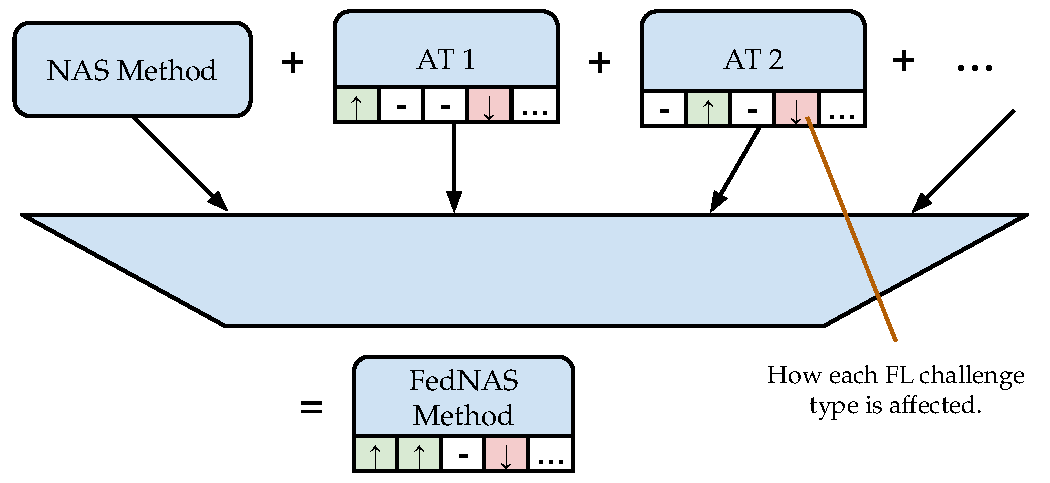
\includegraphics[width=0.7\textwidth]{figures/fednas_method_composition.pdf}
  \caption{A conceptual sketch of how a FedNAS method is composed. \textbf{AT} = adaptation technique.}
  \label{fig:fednas_method_composition}
\end{figure}

Using either NAS or FL on its own is a complex task. Combining them introduces even more possible knobs to turn on the system as a whole. There are many NAS methods for researchers to choose from, and even more potential adaptation techniques to address FL challenges — culminating in a large number of possible FedNAS methods. To understand the current landscape, we ask our first research question:

\vspace{1em}
(RQ1) Which FedNAS methods have been described in the literature, and which adaptation techniques do they use?
\vspace{1em}

As mentioned before, we expect a diverse array of adaptation techniques in the literature. Yet, we also expect some FedNAS methods to use similar adaptation techniques if they address the same type of FL challenges. This leads us to our second research question:

\vspace{1em}
(RQ2) Which adaptation techniques are similar, and what types of challenges of the FL setting do they address?
\vspace{1em}

Adaptation techniques are heavily dependent on the targeted type of FL challenge and the NAS method used. Naturally, this does not allow for most adaptation techniques to work together. Additionally, some adaptation techniques are incompatible due to other reasons. For example, the architecture weight aggregation technique proposed by \cite{efnas_2024} aims to gradually increase the likelihood of sampling the best-performing architectures during training. In contrast, \cite{superfednas_2024} introduces a technique that attempts to maintain a diverse set of architectures throughout the training process. We would still like to know which existing adaptation techniques can be combined in what way, possibly paving the way for creating more powerful FedNAS methods tailored towards specific use cases. This leads us to our third research question:

\vspace{1em}
Optional (RQ3) How can adaptation techniques described in the literature be composed into new, potentially better FedNAS methods?
\vspace{1em}

\section{Methodology}


To address our research questions, we divide our approach into six steps:

\begin{enumerate}
    \item \textbf{Literature Selection:} To tackle the first part of RQ1, we follow the guidelines and flow diagrams provided by PRISMA 2020 \cite{prisma_2020} for inclusion and exclusion of papers and perform forward and backwards citation searching. Each paper presents one or more FedNAS methods. 
    \item \textbf{Adaptation Technique Extraction:} Once the set of included papers is fixed, we tackle the second part of RQ1 by analysing each paper individually, extracting the adaptation techniques it uses and summarising them.
    \item \textbf{Categorise Adaptation Techniques:} For the first part of RQ2, we cluster adaptation techniques based on conceptual similarities and deliver a taxonomy of adaptation techniques.
    \item \textbf{Define FL Challenge Types:} For the second part of RQ2, we must first define a classification of FL challenges. To this end, we repurpose a prior classification \cite{fl_taxonomy_2024} of recent research advances in FL (as shown in \ref{fig:fl_challenge_types_taxonomy}). \cite{fl_taxonomy_2024} suggests that newly proposed FL methods in FL research enhance one or more \textit{evaluation metrics}. We argue that their aforementioned evaluation metrics are the result of finding a measure for how effectively an FL challenge has been addressed. Therefore, the clustering of evaluation metrics into research directions is akin to clustering FL challenges into types of FL challenges.
    \item \textbf{Mapping FL Challenge Types onto Adaptation Technique Clusters:} Next, we review all clusters of adaptation techniques from step 3, and discuss how each adaptation technique cluster works towards, against, or does not affect overcoming each of the FL challenge types defined in step 4.
    \item \textbf{Compose promising FedNAS methods:} For RQ3, we propose building an "is-compatible-with" relation on the set of adaptation technique clusters. We achieve this by cross-examining each adaptation technique cluster with every other one. We then utilise the "is-compatible-with" relation, together with our discussion from step 5, to identify groups of adaptation technique clusters that can be composed into FedNAS methods, which could potentially shift the Pareto frontier with respect to the optimality of addressing FL Challenge types.
\end{enumerate}

\begin{figure}[hbtp]
  \centering
  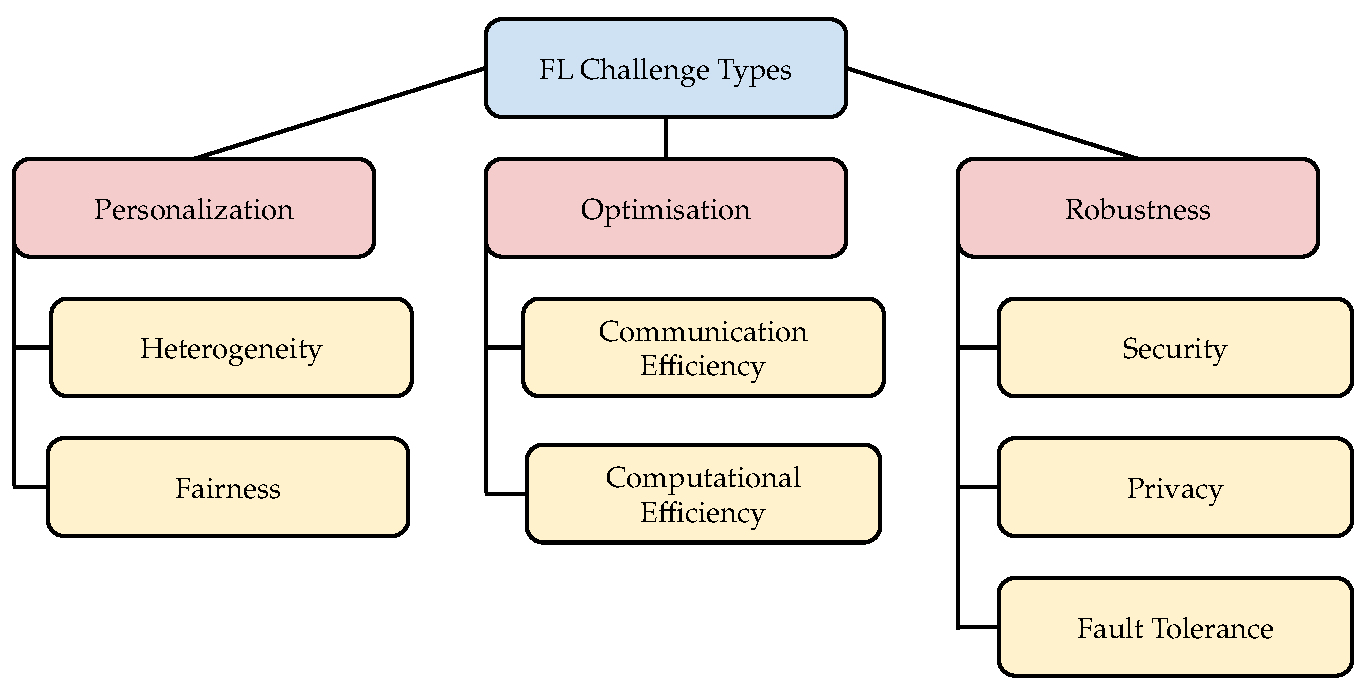
\includegraphics[width=\textwidth]{figures/fl_challenge_types_taxonomy.pdf}
  \caption{A taxonomy of FL challenge types based on \cite{fl_taxonomy_2024}.}
  \label{fig:fl_challenge_types_taxonomy}
\end{figure}